\documentclass{article}%
\usepackage[T1]{fontenc}%
\usepackage[utf8]{inputenc}%
\usepackage{lmodern}%
\usepackage{textcomp}%
\usepackage{lastpage}%
\usepackage{geometry}%
\usepackage{float}%
\usepackage{biblatex}%
\addbibresource{citations.bib}
\geometry{tmargin=3cm,lmargin=2.5cm,rmargin=2.5cm}%
\usepackage{graphicx}%
\setlength{\parskip}{0.5em}%
%
\title{On cosmic and blackbody radiation.}%
\author{Brian Rogers}%
%
\begin{document}%
\normalsize%
\maketitle%
\section{Abstract}%
\label{sec:Abstract}%

This report aims to address two main objectives. Firstly, to verify the Stefan{-}Boltzman law, 
an underpinnnig equation of blackbody radiation theory.
By a chi square test of fit method, we achieve a power law value of $x=4.02 \pm 0.04$ 
and an implied Stefan-Boltzan constant, $\sigma =5.75 \cdot 10^{-8}Wm^{2}K^{-4} $. 
These results are consistent with existing consensus values. \par
Secondly, we measure the temperature of the cosmic background radiation. These photons permeate the universe and
provide key evidence of the 'big bang' theory.  By analysis of the data collected during the COBE experiment, 
we estimate that the background radiation follows a blackbody distrubution with a temperature of $T = 2.73K \pm 0.00546K$.
This is consistent within the uncertainties with measured by the COBE experiment. 

%
\section{Introduction}%
\label{sec:Introduction}%

Blackbody radiation has played an integral role in modern physics.
Inconstitencies with a theoretical blackbody and classical electromagnetic theory
led Max Planck to consider the quantization of energy and laid the ground work for the oncoming "Quantum Revolution".\cite{Baggot}
For his work, Planck recieved the Nobel prize in 1919.
In addition to it's role on the quantum scale, blackbody radiation has had an important contributions to astrophysics.
Penzias and Wilson detected cosmic microwave background radiation and found it consistent with a blackbody
at temperature T=3K. This was confirmed by the COBE satellite launched in 1989 which confirmed that 
the CMBR had a perfect blackbody spectrum with T=2.73K. Both scientific endeavours earned the Noble prize in 1978 and 2006 respectively.  


The radiance for a blackbody as a function of wavelength, $\lambda$ and temperature, T is as follows:
\begin{equation}
  \resizebox{.3\hsize}{!}{$I_{\lambda}(\lambda,T) = \frac{2hc^2}{\lambda^5 (e^ \frac{hc}{\lambda kT} - 1)}$}
  \end{equation}
Simulating a theoretical blackbody spectrum at wavelength intervals of 10nm you can generate the following 
curve for T=5780K.


\begin{figure}[H]%
\centering%
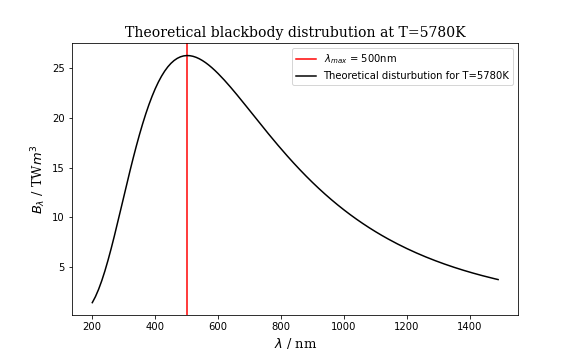
\includegraphics[width=300px]{task1_fig_a.png}%
\caption{Example theoretical plot of a blackbody emission distrubution for T=5780K}%
\end{figure}


The corresponding maximum wavelength, $\lambda_{max}$ = 500nm. Comapring this to Wien's law which states: 

\begin{equation}
   \lambda_{max} = \frac{b}{T}
\end{equation}



Where $b=2.90 \cdot 10^-3$ mK . Wien's law yields $\lambda_{max}$ = 501nm. 
This confirms our expectations for the theoretical spectrum. 


Using a halogen lamp as a source and a spectrograph connected to the Spectralab software we compare our theoretical blackbody simulation
to a physical approximation of a blackbody. 

\begin{figure}[H]%
\centering%
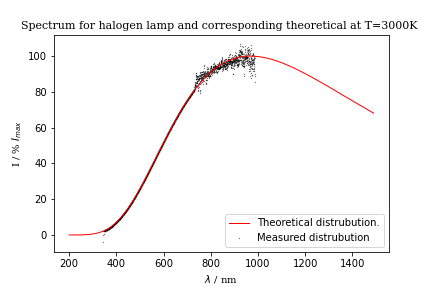
\includegraphics[width=300px]{task3_fig_a.png}%
\caption{Comparison of theoretical blackbody spectrum and a spectrum produced by a blackbody at T=3000K}%
\end{figure}


The spectrograph had a dection limit of $360nm < \lambda < 1000nm$. However within theses limits clear aggrement between the theoretical and experimental curves is demonstrated.
With confidence in the theoretical simulation, we preceeded to the address the key objectives of our experiment.

%
\section{Verification of the Stefan{-}Boltzman law}%
\label{sec:VerificationoftheStefan{-}Boltzmanlaw}%
%
\subsection{Methodology}%
\label{subsec:Methodology}%
We used a halogen lamp as a light source powered by a variable power supply. 
Using a a connected voltmeter and ammeter, we calculated the power by the source to be:

\begin{equation}
  P = IV
\end{equation}


We used voltage values ranging from 12V to 6V at 1V intervals.
After accounting for background effects and incorporating the sensitivity of the spectrogrpah for the relevant exposure time,
we used the fitting software on Spectralab to record the temperature of the source. 
We repeated this for both wavelength and frequency regimes to 
gain additional temperature data and calculate an 
average temperature value for specific power values.\par


Once the data was collected we could begin to analyse the results. Starting with the Stefan-Boltzman law with the unknown exponent:
\begin{equation}
  P = \sigma T^x\
\end{equation}
where $ \sigma $ is the Stefan-Boltzman constant and x is the constant to be determined. \par

Converting this equation into linear form we get:
\begin{equation}
  \ln(P) = ln(\sigma) + x \ln(T)
\end{equation}

A plot of $\ln(P)$ on $\ln(T)$ yields a linear curve with gradient x and y-intercept of $\ln(\sigma)$ \par

%
\subsection{Results and analysis}%
\label{subsec:Results and analysis}%
Using our theoretical blackbody model, it was possible to compare observed values for the radiance to the expected theoretical values.
A chi square method was used to calculate the optimal value of $x=4.02 \pm 0.04$. The plot belows shows the optimal value occuring at the minimum of the graph. 

\begin{figure}[H]%
    \centering%
    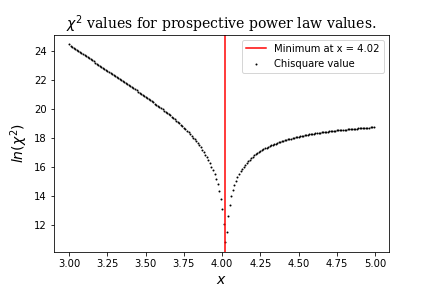
\includegraphics[width=300px, height=150px]{task4_fig_a.png}%
    \caption{Iterations of $\chi^2$ value for a range of temperature values used with equation (5)}%
    \end{figure}

The experimental results are as follows with associated line of best fit determined from the chi sqaure fit process from above.
\begin{figure}[H]%
  \centering%
  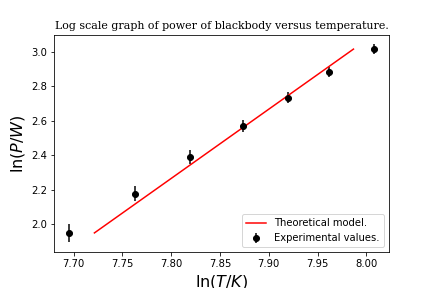
\includegraphics[width=300px]{task4_fig_b.png}%
  \caption{Power on Temperature on a natural log scale}%
  \end{figure}

  Interpretting the y-intercept value as $\ln(\sigma)$, we get $\sigma = 5.75 \cdot 10^{-8} Wm^{-2}K^{-4}$ 

%
\subsection{Discussion}%
\label{subsec:Discussion}%
The experimental values are in broad agreement with the currently accepted values. The exponent value of x=4.02 $\pm 0.04$
agrees with derived value of x=4 \cite{Boltzman}. Whilst the implied Stefan-Boltzman constant has an error of +1.39\%. \cite{Martin}
Limitations in our experimental method can explain in part why our values deviate above the accepeted values. \par

During the experiment, noise detected on the intensity of the higher wavelengths increased significantly, making it more diificult
to obtain a stable value for the temperature. We attempted to use a higher integration time but this often caused the software to crash.
By using a computer with higher processing power we could obtain a higher resolution spectrum. \par

Further, error may be induced by not incorporating the efficiency of the lamp. An efficiency of less than 1 would mean that power values used
are overestimated. This is visible by close up inspection of a figure 2, where the intensity values are lower for each frequency. By changing equation (3) used to calculate power to:

\begin{equation}
  P = \eta I V
\end{equation}
Where $\eta$ is the efficiency of the lamp, we could obtain a more accurate value for x and $\sigma$. \par

We could also attribute error to fluctuations in the background radiation. By increasing the number of times we correct for background radiation, we could improve our measurements. 
An alternative would be to enclose the lamp in opaque box and remove any background fluctuations in the visible region. \par
%

%
\section{Measurement of the temperature of the cosmic background radiation}%
\label{sec:Measurementofthetemperatureofthecosmicbackgroundradiation}%
%
\subsection{Methodology}%
\label{subsec:Methodology}%
We used a Chi square fit method to determine the optimal temperature value for the COBE dataset,
again utilising our theoretical simulation for the blackbody for a range of temperature values.
The minimum chi square value corresponded to a temperature of T=2.71K. It was then possible to generate the best fit curve for the COBE dataset.
%
\subsection{Results and analysis}%
\label{subsec:Analysis}%
The chi square values can be shown for various temperature values. \par
\begin{figure}[H]%
\centering%
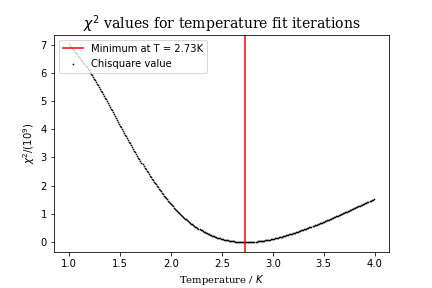
\includegraphics[width=300px]{task5_fig_b.png}%
\caption{Plot of Chi square values obtained from comparing our COBE dataset and theoretical blackbody simulation. $\chi^2_{min}$ yields T = 2.71K }%
\end{figure}
%
The corresponding best curve fit can then be plotted:
\begin{figure}[H]%
\centering%
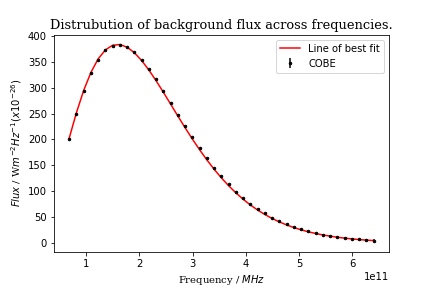
\includegraphics[width=300px]{task5_fig_a.png}%
\caption{COBE experimental data with line of best fit obtained by the chi square method.}%
\end{figure}

%
\subsection{Discussion}%
\label{subsec:Discussion}%
In comparison with the Mather et. al our value in is broad agreement with their result of T=2.725 $\pm$ 0.06K \cite{Mather}.
However, we lack the accuracy of their measurement. This is primarily due to the fact that the subset of that we use has 42 measurements.
By obtaining and using a larger dataset, we could improve the accuracy of our measurement. \cite{github} \par

%

%
\section{Conclusion}%
\label{sec:Conclusion}%
We have addressed both our objectives: to verify the Stefan-Boltzman law and to measure the cosmic microwave background radiation.
Although broad agreement has been demonstrated with the currently accepted measurements, we have suggested a number of improvements to our experimental and analytical methods for future experimentation. \par
%
\printbibliography 

%
\end{document}